\section{Creación de un nuevo Issue mediante GitHub CLI}

Una vez verificado el acceso al repositorio, se procedió a crear una nueva incidencia desde la terminal utilizando el siguiente comando:

\begin{lstlisting}
gh issue create \
--repo martinezmoralesdiego2020-droid/repositorio \
--title "Error al guardar datos" \
--body "El sistema no guarda correctamente la informacion ingresada por el usuario."
\end{lstlisting}

El comando generó correctamente el Issue \#8 dentro del repositorio.

\begin{figure}[H]
\centering
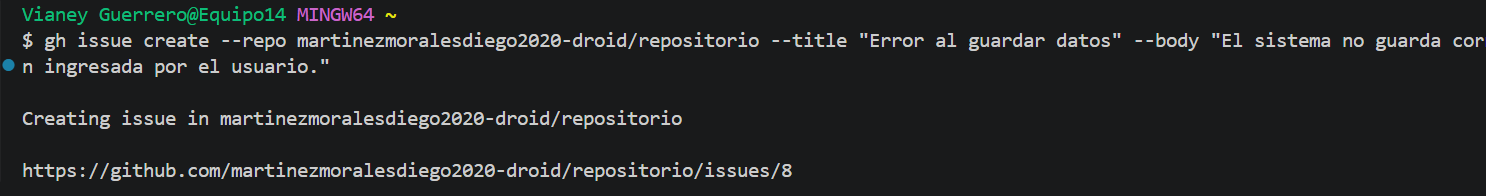
\includegraphics[width=0.9\textwidth]{M6.png}
\caption{Creación del Issue ``Error al guardar datos'' mediante GitHub CLI.}
\end{figure}

Posteriormente se volvió a consultar el listado de incidencias, observándose que el nuevo Issue aparecía registrado junto con los anteriores.

\begin{figure}[H]
\centering
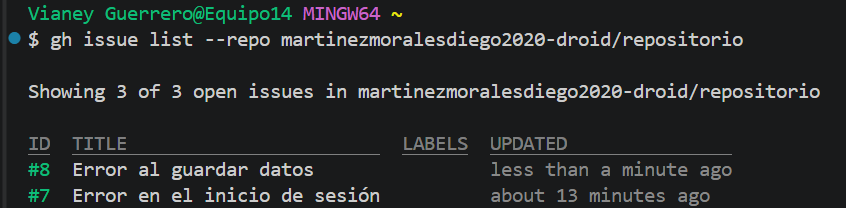
\includegraphics[width=0.9\textwidth]{M7.png}
\caption{Listado actualizado de Issues después de crear la nueva incidencia.}
\end{figure}
